\documentclass[11pt,a4paper]{article}
\usepackage[utf8]{inputenc}
\usepackage[T1]{fontenc}
\usepackage[french]{babel}
\usepackage[a4paper,margin=2.2cm]{geometry}
\usepackage{booktabs}
\usepackage{hyperref}
\usepackage{microtype}
\usepackage{pdfpages}
\usepackage{tabularx}
\usepackage[most]{tcolorbox}
\usepackage{xcolor}

\definecolor{ink}{HTML}{202124}
\definecolor{muted}{HTML}{5F6368}
\definecolor{line}{HTML}{DADCE0}
\definecolor{paper}{HTML}{F8F9FA}
\definecolor{green}{HTML}{0B6B57}
\definecolor{greensoft}{HTML}{E6F4EF}
\definecolor{blue}{HTML}{245B8E}
\definecolor{bluesoft}{HTML}{EAF2FA}
\definecolor{accent}{HTML}{8A1538}

\hypersetup{colorlinks=true,linkcolor=accent,urlcolor=accent,hypertexnames=false}

\begin{document}

\begin{titlepage}
\centering
\vspace*{1.4cm}
{\color{accent}\rule{0.86\linewidth}{1.1pt}\par}
\vspace{0.8cm}
{\Huge\bfseries\color{ink} Python pour économistes\par}
\vspace{0.35cm}
{\Large Livret de TD appliqués avec Our World in Data -- version révisée\par}
\vspace{0.75cm}
{\large Université de Lille -- L2 Économie\par}
\vspace{0.2cm}
{\large Année 2026--2027\par}
\vspace{1.1cm}
\begin{tcolorbox}[
  enhanced,
  width=0.86\linewidth,
  colback=paper,
  colframe=line,
  boxrule=0.6pt,
  arc=2pt,
  left=12pt,right=12pt,top=10pt,bottom=10pt,
  borderline west={3pt}{0pt}{accent}
]
Ce livret rassemble les cinq TD. Chaque séance articule apprentissage de Python, statistiques descriptives simples, pseudo-code et applications économiques fondées sur des données Our World in Data.
\end{tcolorbox}
\vspace{0.4cm}
\begin{tabularx}{0.86\linewidth}{@{}>{\bfseries\color{accent}}p{0.28\linewidth}X@{}}
Obligatoire & exercices à rendre et résultats attendus.\\
Pseudo-code & étapes à compléter avant d’écrire le Python.\\
Pathways & chemins de fichiers, dossiers courants et sorties reproductibles.\\
Compléments & entraînement supplémentaire pour consolider la séance.
\end{tabularx}
\vfill
{\color{muted}Objectif : apprendre Python en transformant progressivement des indicateurs économiques OWID en scripts clairs, graphiques et interprétations prudentes.\par}
\vspace{0.4cm}
{\color{accent}\rule{0.86\linewidth}{1.1pt}\par}
\end{titlepage}

\phantomsection
\addcontentsline{toc}{section}{Mode d’emploi du livret}
\section*{Mode d’emploi du livret}
\begin{tcolorbox}[
  enhanced,breakable,
  colback=bluesoft,
  colframe=blue,
  coltitle=ink,
  title={Comment travailler une séance},
  fonttitle=\bfseries,
  boxrule=0.6pt,
  arc=2pt,
  left=9pt,right=9pt,top=7pt,bottom=7pt,
  borderline west={2.6pt}{0pt}{blue}
]
\begin{enumerate}
  \item Lire la question fil rouge, la source OWID et les livrables avant de coder.
  \item Compléter le pseudo-code : données, étapes Python, sortie statistique, contrôle.
  \item Écrire le script par petits blocs et l’exécuter souvent.
  \item Vérifier les chemins de fichiers, surtout le dossier courant et le dossier \texttt{out}.
  \item Quand une erreur apparaît, lire la dernière ligne, identifier le type d'erreur, puis revenir à la ligne indiquée.
  \item Terminer par une interprétation courte, prudente et reliée aux résultats économiques.
\end{enumerate}
\end{tcolorbox}

\tableofcontents
\clearpage

\phantomsection
\addcontentsline{toc}{section}{TD1 -- Premiers scripts et statistiques descriptives simples}
\hypersetup{pageanchor=false}
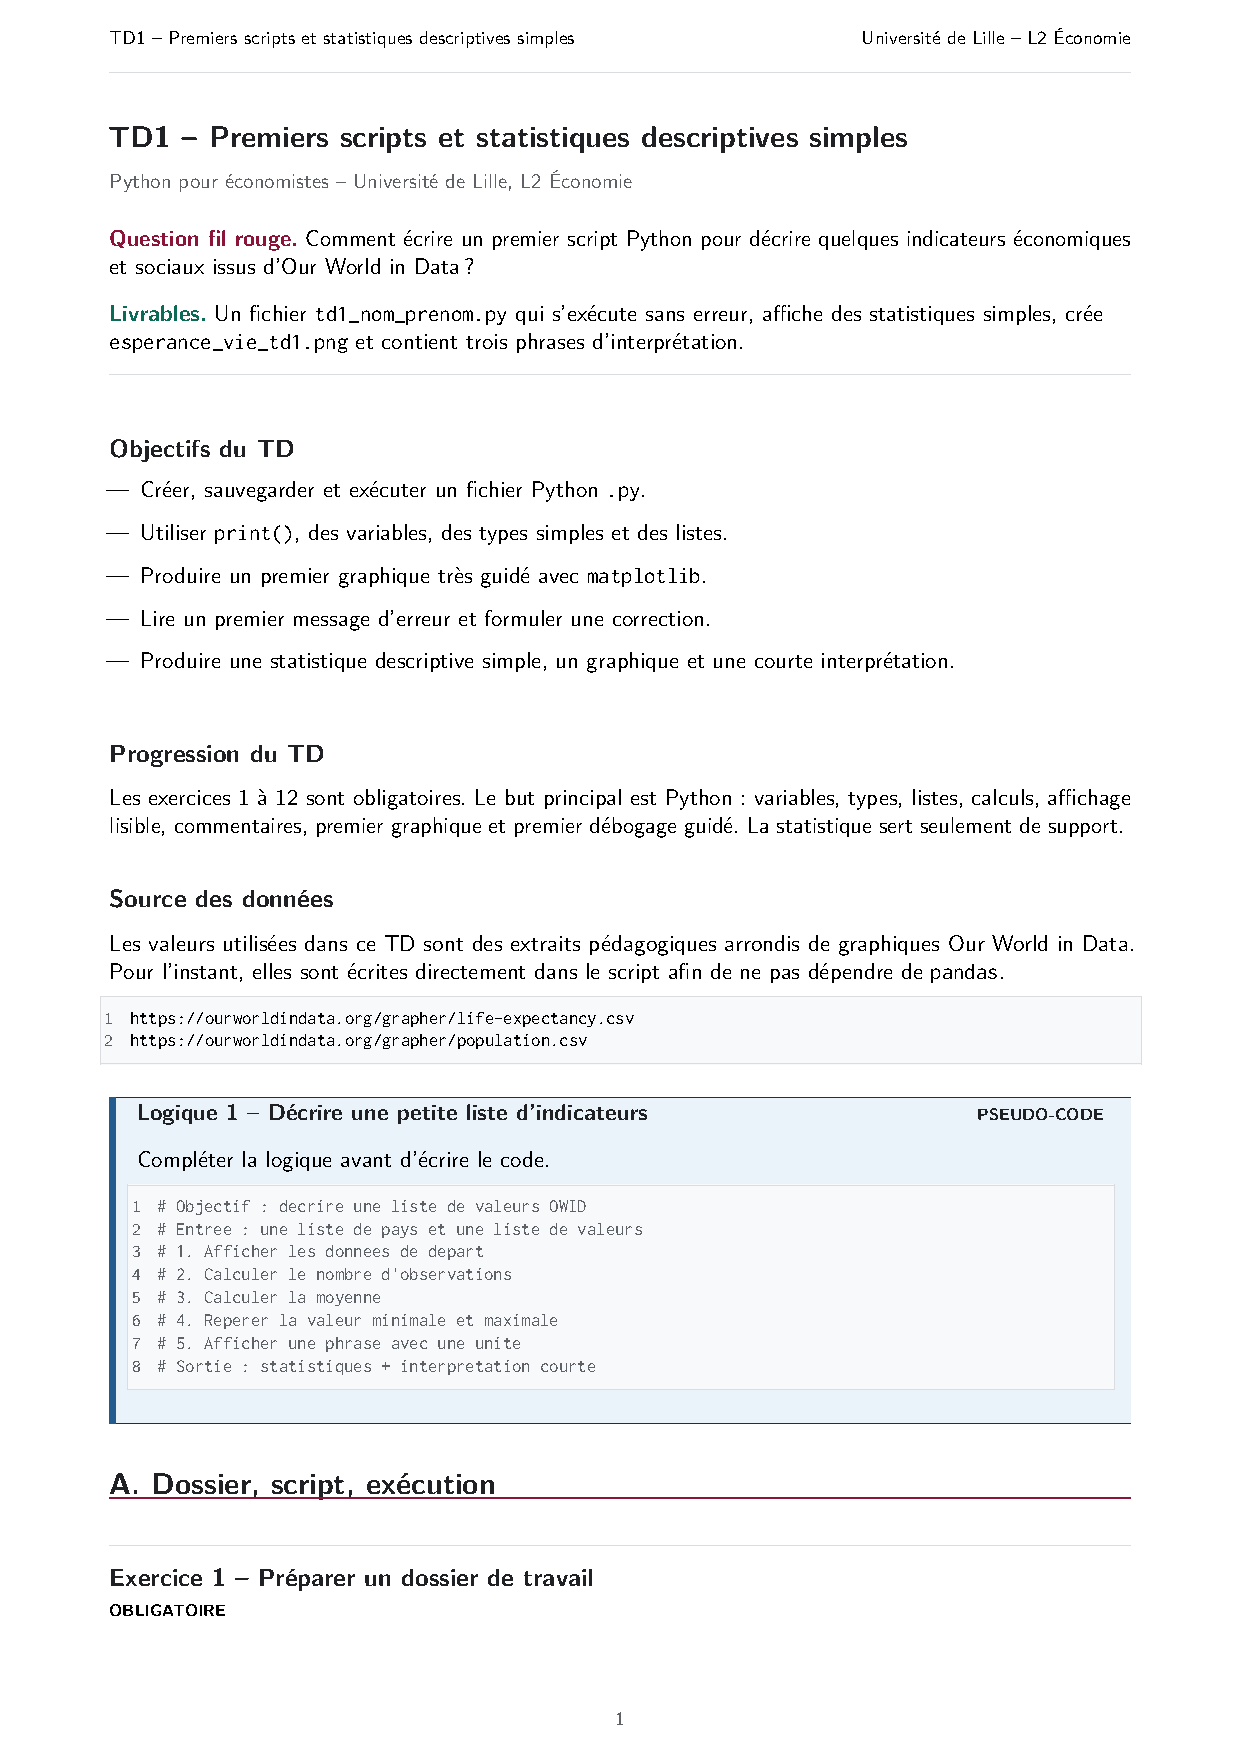
\includepdf[pages=-]{seance_3/TP_1_revise.pdf}
\hypersetup{pageanchor=true}

\phantomsection
\addcontentsline{toc}{section}{TD2 -- Boucles, conditions et proportions avec données OWID}
\hypersetup{pageanchor=false}
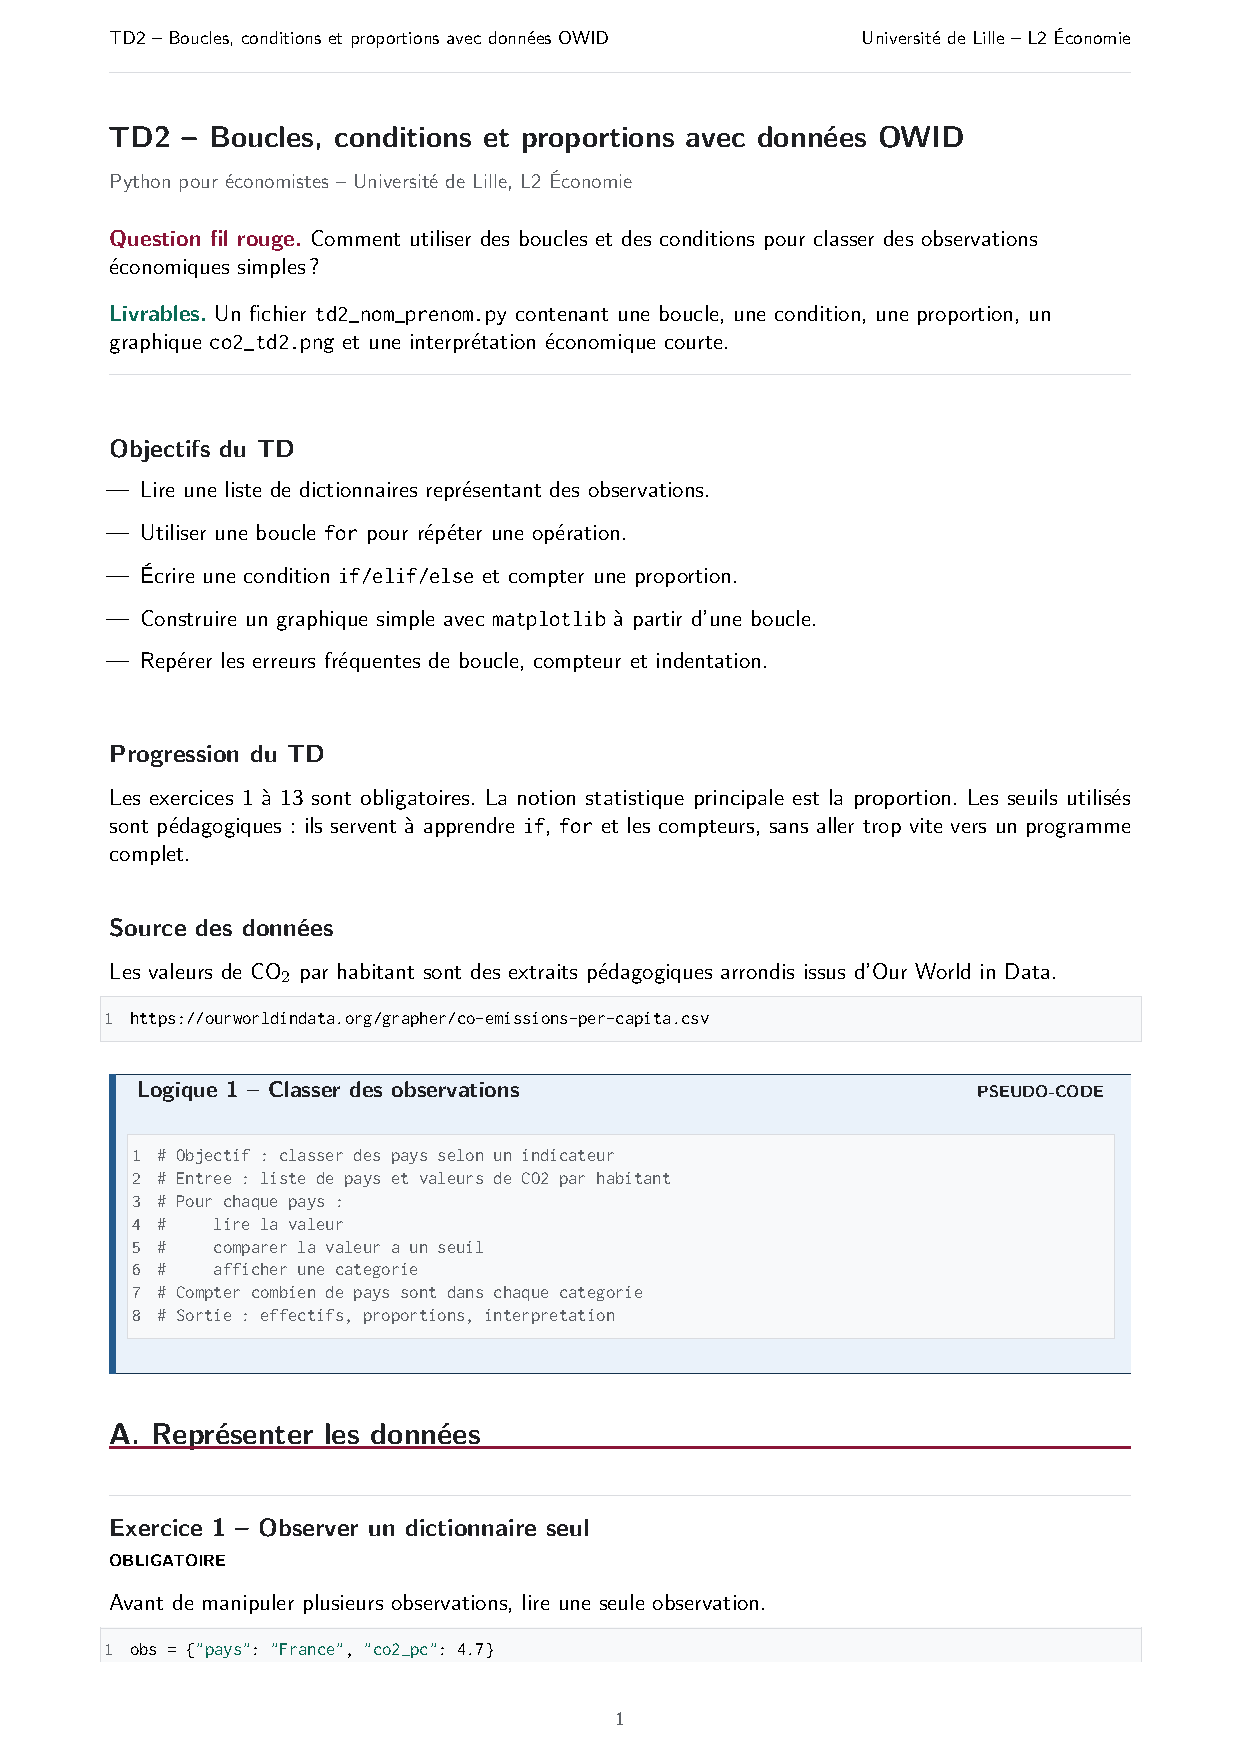
\includepdf[pages=-]{seance_4/TP_2_revise.pdf}
\hypersetup{pageanchor=true}

\phantomsection
\addcontentsline{toc}{section}{TD3 -- Fonctions et comparaison de groupes}
\hypersetup{pageanchor=false}
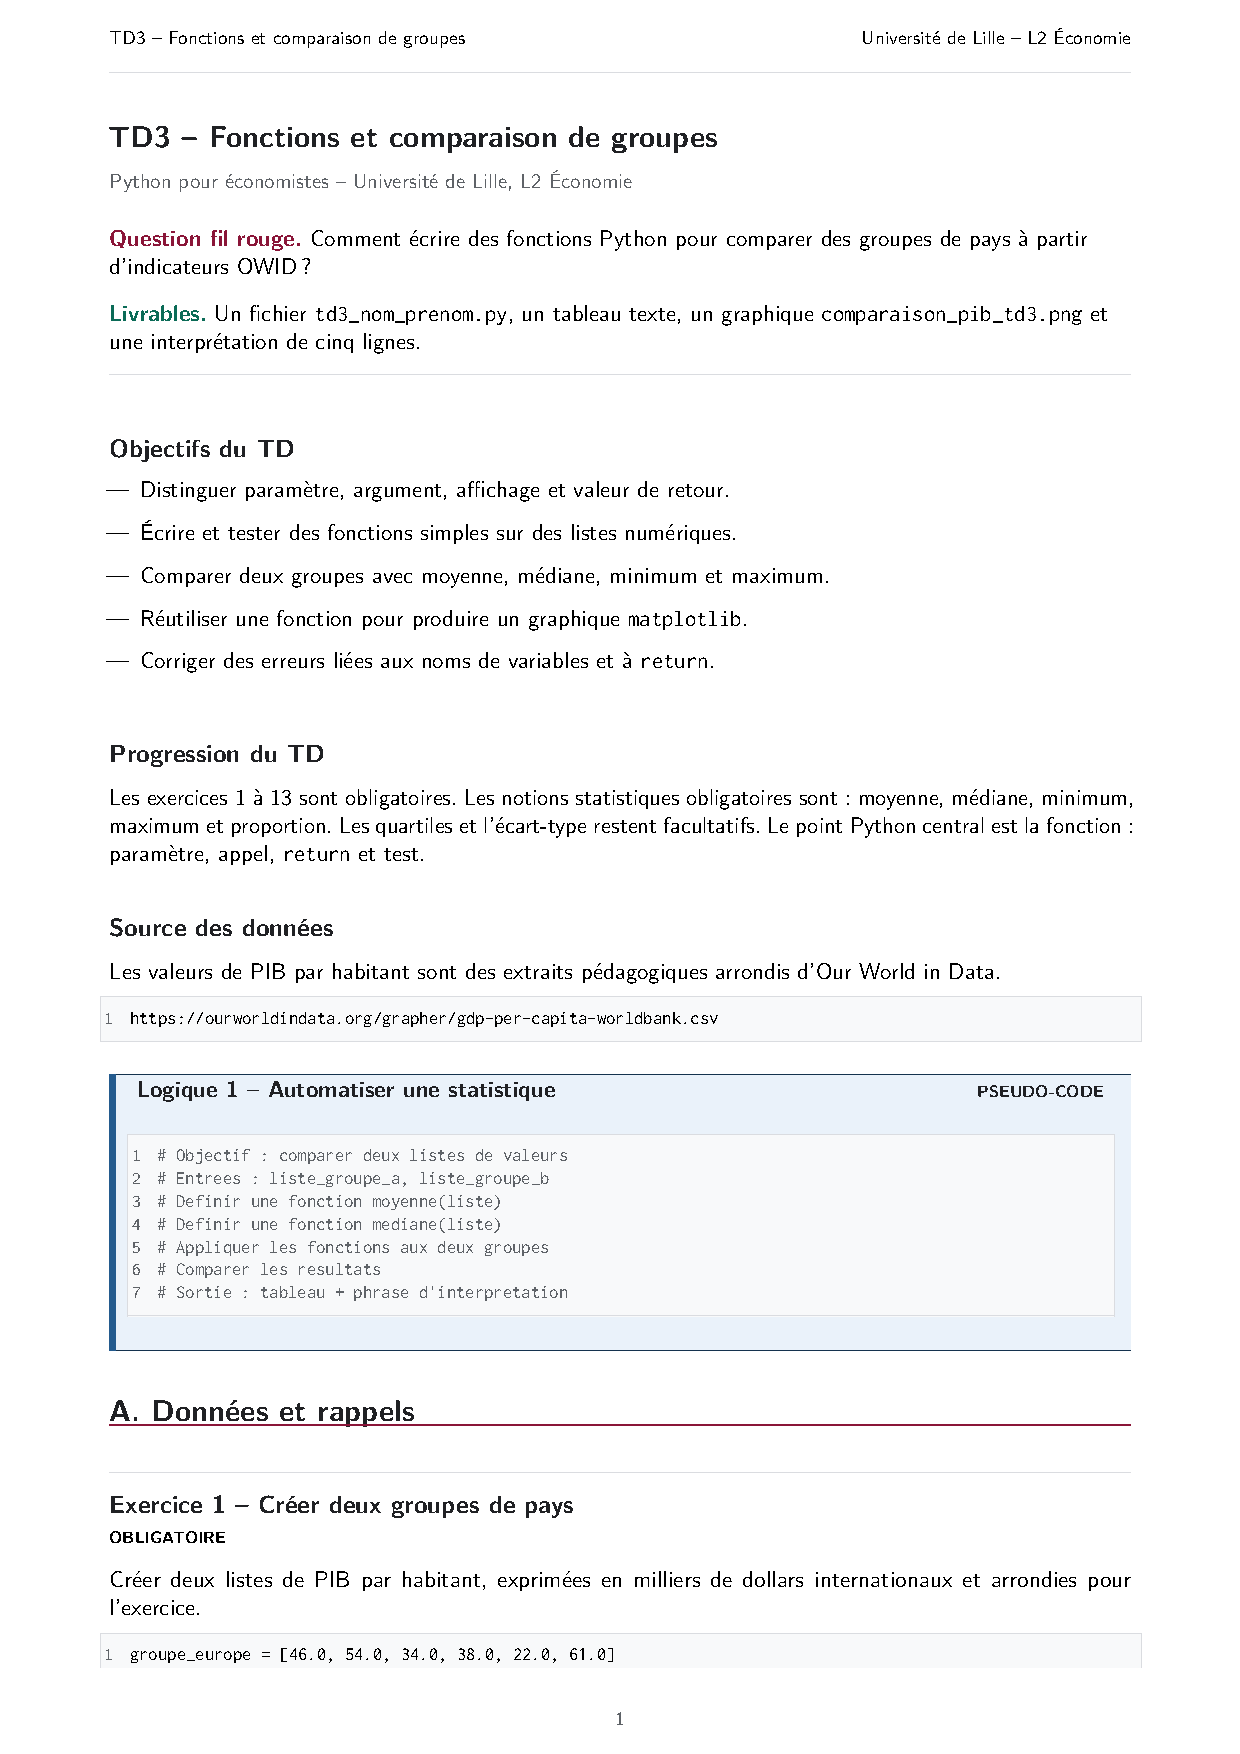
\includepdf[pages=-]{seance_5/TP_3_revise.pdf}
\hypersetup{pageanchor=true}

\phantomsection
\addcontentsline{toc}{section}{TD4 -- Graphiques et simulation simple à partir d'OWID}
\hypersetup{pageanchor=false}
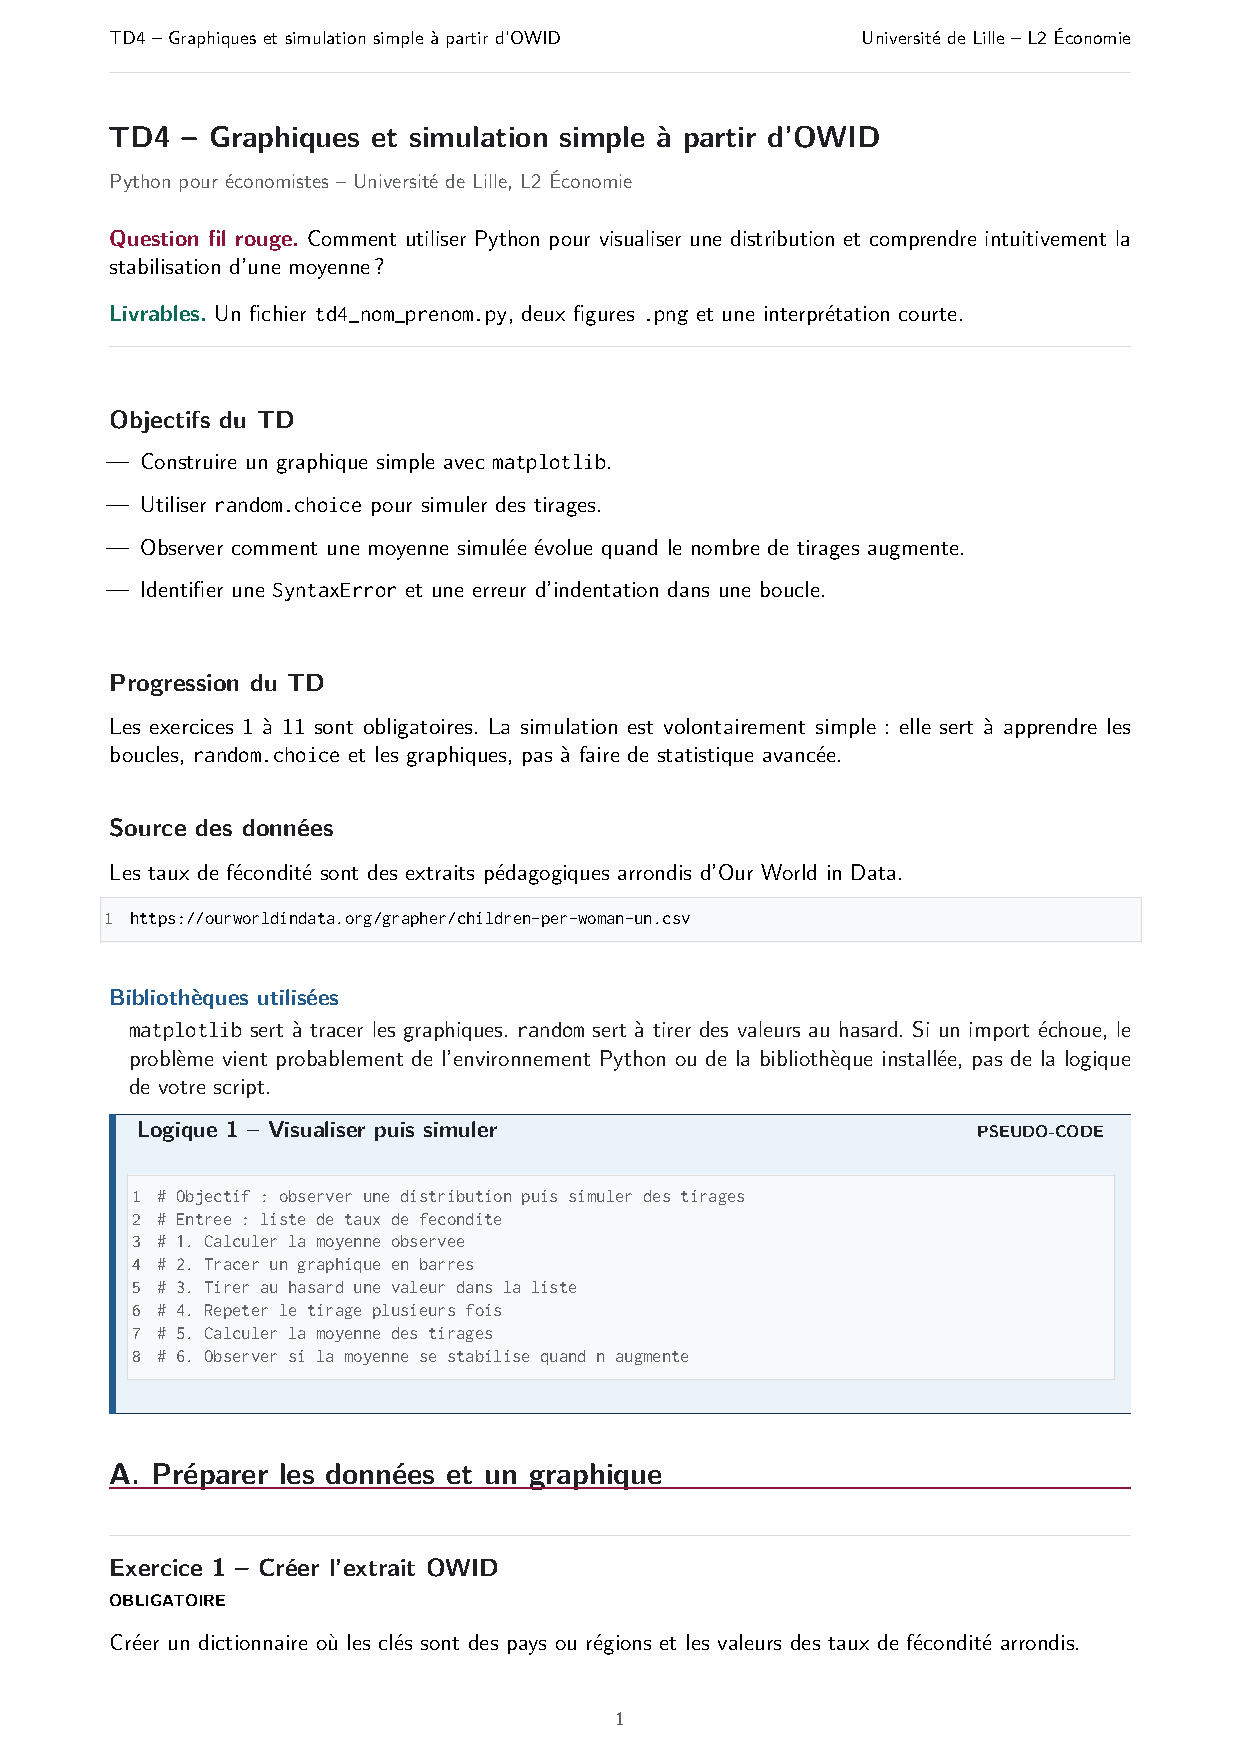
\includepdf[pages=-]{seance_6/TP_4_revise.pdf}
\hypersetup{pageanchor=true}

\phantomsection
\addcontentsline{toc}{section}{TD5 -- Mini-projet pandas avec Our World in Data}
\hypersetup{pageanchor=false}
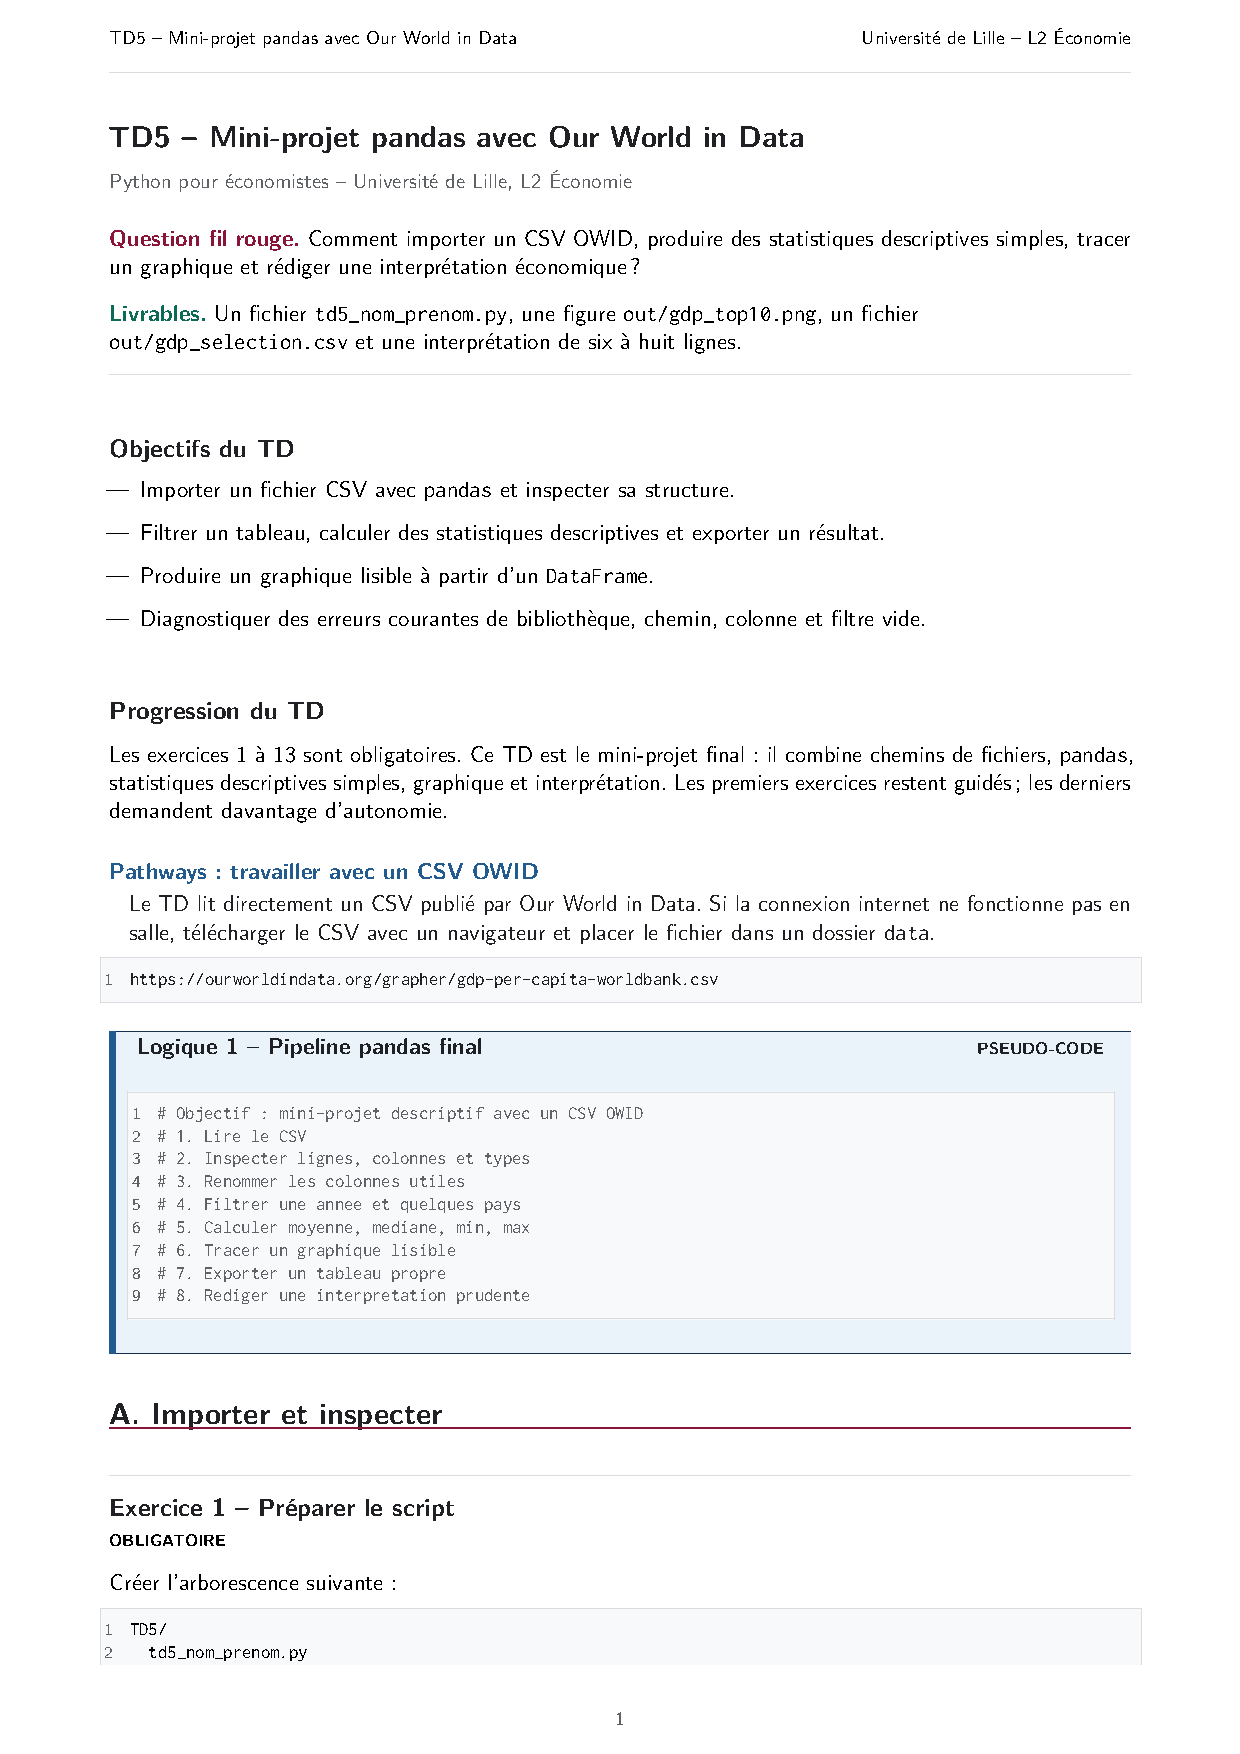
\includepdf[pages=-]{seance_7/TP_5_revise.pdf}
\hypersetup{pageanchor=true}

\end{document}
